% !TeX root = RJwrapper.tex
\title{\pkg{lagr}: Local Adaptive Grouped Regularization in R}
\author{Wesley Brooks}

\maketitle

Whereas the coefficients in traditional linear regression are constant, the coefficients in a varying coefficient regression (VCR) model are functions - often smooth functions - of some effect-modifying parameter \citep{Cleveland-Grosse-1991,Hastie-Tibshirani-1993}. A basic fact of varying coefficient regression (VCR) models is that the coefficients vary over the model's domain. It is natural, then, to allow that a coefficient function may be nonzero in part of the domain and exactly zero elsewhere. This paper introduces \pkg{lagr}, an R package for estimating a VCR model via LAGR. The method of LAGR is described, some features of the software are explained, and the results are illustrated with an example application.

\section{Method}
A brief overview of LAGR follows. It can be shown that under some mild conditions the method achieves an oracle property, asymptotically identifying exactly the locally relevant covariates and estimating them as accurately as if their identities were known in advance \citep{Brooks-Zhu-Lu-2014}.

\subsection{Varying coefficient regression}
The response $Y(s)$, covariates $\bm{X}(s)$, and coefficients $\bm{\beta}(s)$ in a VCR model are indexed by the location parameter $s$. Assume $n$ observations of the response and the covariates at locations $s_1, \dots, s_n$ and let $Y_i = Y(s_i)$, $\bm{X}_i = \bm{X}(s_i)$, and $\bm{\beta}_i = \bm{\beta}(s_i)$. The generalized linear model (GLM) with varying coefficients is written
\begin{align*}
	E[Y(s)|\bm{X}(s)] &= \mu(s)\\
	\eta(s) = g(\mu(s)) &= \bm{X}'(s) \bm{\beta}(s)\\
	\text{var}[Y(s)|\bm{X}(s)] &= \phi V(\mu(s))
\end{align*}
where $g(\cdot)$, $V(\cdot)$, and $\phi$ are, respectively, the link function, variance function, and dispersion parameter of the response family. For simplicity of notation, assume the canonical link function \citep{McCullagh-Nelder-1989}.

\subsection{Local polynomial regression}
Local adaptive grouped regularization is in the class of local polynomial regression methods. At each estimation location $s_i$, the coefficient functions are approximated by Taylor's expansion as locally linear functions of the location parameter
\begin{equation}\label{eq:taylors}
\bm{\beta}(s) = \bm{\beta}(s_i) + \nabla \bm{\beta}(s_i) (s - s_i) + o(|s-s_i|).
\end{equation}
The locally linear approximation is implemented by augmenting the matrix $\bm{X}(s)$ with interactions between the covariates and the location parameter. Letting $\bm{Z}(s) = \left( \bm{X}_i \; (s-s_i)\cdot\bm{X}_i \right)$ and $\bm{\zeta}(s) = (\bm{\beta}(s)^T, \; \nabla \bm{\beta}(s)^T)^T$, the linear predictor of the local GLM is $\hat{\eta}_i = \bm{Z}_i \bm{\zeta}_i$.

Weights are calculated according to a kernel function that gives more weight to nearby observations than to distant ones. The popular Epanechnikov kernel is defined as \citep{Samiuddin-el-Sayyad-1990}:
\begin{equation*}
K(x) = (3/4) (1-x^2) \text{ if } x<1, \text{ and } 0 \text{ otherwise}.
\end{equation*}
Because the kernel gives zero weight to observations farther than $h$ from the estimation location, the error term in \eqref{eq:taylors} is small.

Let $\delta$ be the dimension of the location parameter (e.g., $\delta=1$ for a coefficients that vary with time). For estimation at location $s_i$ with kernel function $K(\cdot)$ and bandwidth $h$, the weights are $w_{ij} = h^{-\delta} K(|s_i-s_j|)$ for $j = 1, \dots, n$. 

\subsection{Penalized local quasi-likelihood}
The quasi-likelihood $Q(\mu, Y)$ is an approximation to the full log likelihood. Its derivative the quasi-score function is $q(\mu, Y) = (y-\mu) \{V(\mu)\}^{-1}$, which is a function of the linear predictor $\eta$ through the link and variance functions. The method of LAGR estimates the coefficients of a VCR model by maximizing the penalized local quasi-likelihood $\mathcal{J}(\bm{\beta}_i; \lambda_i)$, which incorporates the local kernel weights and an adaptive group lasso penalty. 

The penalized local quasi-likelihood is
\begin{align*}
\mathcal{J}(\bm{\beta}_i; \lambda_i) &= \ell(\bm{\beta}_i) - \mathcal{P}(\bm{\beta}_i; \lambda_i) \\
&= \sum_{j=1}^n w_{ij} Q(\hat{\mu}_i, Y_j) - \lambda_i \sum_{k=1}^p \gamma_{ik} \| \bm{\zeta}_{i(k)} \|
\end{align*}
where $\| \bm{\zeta}_{i(k)} \| = \{ \left(\beta_k(s_i), \; \nabla \beta_k(s_i)\right)^T \left(\beta_k(s_i), \; \nabla \beta_k(s_i)\right) \}^{1/2}$ is the norm of the $k$th coefficient group, which consists of the $k$th coefficient and its interaction with the location parameter. The penalty on the norm of the $k$th covariate grouping is a combination of $\gamma_{ik}=\| \tilde{\zeta}_k(s_i) \|^{-1}$, an adaptive penalty based on the unpenalized local coefficients $\tilde{\zeta}_k(s_i)$; and $\lambda_i$, a local tuning parameter estimated by the Akaike Information Criterion (AIC) \citep{Akaike-1973}.


\section{Package}
The R package \pkg{lagr} (\url{https://github.com/wrbrooks/lagr}) estimates a VCR model via LAGR. The primary functions of the package are \code{lagr} and \code{lagr.tune}. The \code{lagr} function estimates a model by LAGR, while the \code{lagr.tune} function estimates profiles the bandwidth parameter with respect to a model selection criterion.

\subsection{Coefficient estimation}
Estimation is carried out by blockwise coordinate descent. Each block is a covariate group, consisting of a raw covariate and its interaction with the location parameter. Coordinate descent is an iterative algorithm; a compiled library can achieve a significant speedup over pure R. The \pkg{lagr} package makes use of a coordinate descent algorithm written in C++ and integrated via the \pkg{Rcpp11} package.

By default, a local model is estimated at each observation location. Since each local model is estimated independently of the others, estimation of a VCR model by LAGR is an embarrassingly parallel problem. The package is written to take advantage of multicore parallelism via the R packages \pkg{foreach} and \pkg{doMC}.

\subsection{Bandwidth parameter estimation}
Two types of bandwidth parameter are supported by the \pkg{lagr} package. The user may specify the bandwidth directly, in which case the \code{bw} function argument is used as $h$ in the kernel function. Alternatively,  $k$-nearest neighbors (KNN) is a type of adaptive bandwidth that allows $h$ to differ among the local models. Specifically, if a KNN bandwidth is specified as $\alpha$, then the bandwidth for the local model at $s_i$ is set so that $\alpha = \sum_{j=1}^n w_{ij}$.

Both types of bandwidth provide a tuning parameter than must be estimated. In the case of the raw bandwidth, that parameter is $h$, and in the case of $k$-nearest-neighbors, that parameter is $\alpha$. In either case, the function \code{lagr.tune} calls R's \code{optim} function to find the bandwidth parameter that minimizes a selection criterion (AIC, BIC, or GCV). 

\subsection{Response family}
R provides several \code{family} objects representing exponential family distributions (e.g., \code{gaussian()}, \code{binomial()}, \code{poisson()}). These objects supply the link and variance functions for estimating the local models. Because the \pkg{Rcpp11} package provides seamless R and C++ integration we can use objects of type \code{Function} within the C++ code to represent either R or C++ functions. This capability allows us to call the \code{link()} and \code{varfun()} functions of any \code{family} object from within compiled C++ code, even a user-provided \code{family} object written in pure R.

\subsection{Plotting}
The function \code{lagr.plot} is used to plot a \code{lagr} object. In the case of a one-dimensional location parameter (e.g., time), the function produces line plots. If the location parameter is two-dimensional, then the plotting behavior depends on how the data was specified. If data was provided as a \code{SpatialPolygonDataFrame} (defined in package \pkg{sp}), then the spatial polygons are used to produce a choropleth (Figure \ref{fig:georgia}). Otherwise the estimation locations are used to generate a Voronoi diagram.

The content of the plot depends on two parameters. The parameter \code{type} is one of \code{raw}, \code{coef}, or \code{is.zero}; these respectively output the raw covariate, the estimated coefficient, or the confidence that a coefficient is locally zero. The parameter \code{target} indicates which covariate is plotted.

\section{Example - Georgia educational attainment data}
We illustrate the functionality of \pkg{lagr} with an example. The dataset \code{georgia} is attached to the package \pkg{lagr}. Here we produce a model for how some demographic covariates are related to educational attainment in Georgia, based on data from the 1990 U.S. Census \citep{Fotheringham-Brundson-Charlton-2002}. The variables in the data set are listed in Table \ref{table:georgia-data}. In this example, the response is the PctBach, the percentage of residents in each county who have at least a bachelor's degree.

\begin{table}[h]
	\centering
	\begin{adjustbox}{max width=\textwidth}
	\begin{tabular}{ll}
	Name & Description \\
	\hline
	Latitude, Longitude & Latitude and longitude of each county's center of mass \\
	PctBach & Percentage of residents with at least a bachelor's degree\\
	PctRural & Percentage of residents living in a rural area\\
	PctEld & Percentage of residents age 65 or older\\
	PctFB & Percentage of residents who are foreign-born \\
	PctPov & Percentage of residents living in poverty \\
	\end{tabular}
	\end{adjustbox}
	\caption{Listing of the variables for each county of Georgia in the example data set. The response for our model is PctBach and the coordinates are given by Longitude and Latitude.
	\label{table:georgia-data}}
\end{table}

\begin{figure}
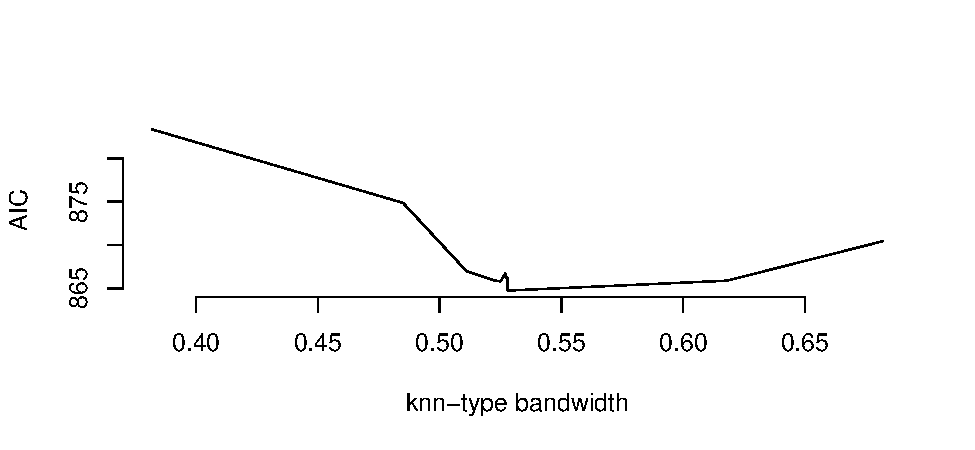
\includegraphics[width=\textwidth]{figure/AIC.pdf}
\caption{Profile AIC for estimating the bandwidth parameter in the Georgia educational attainment model. The AIC is minimized for $k$-nearest-neighbors bandwidth parameter $0.525$.}
\label{fig:AIC}
\end{figure}

In the code listed below, we import the data and estimate the bandwidth by AIC, then fit a model using the estimated bandwidth. The profile AIC of the bandwidth estimation is shown in Figure \ref{fig:AIC}, showing that the optimal $k$-nearest-neighbors bandwidth for the example is $0.525$. 

\begin{example}
library(lagr)
data(georgia)

bw = lagr.tune(PctBach~PctRural+PctEld+PctFB+PctPov, data=georgia,
    bw.type='knn', bwselect.method='AIC', longlat=TRUE,
    kernel=epanechnikov)

model = lagr(PctBach~PctRural+PctEld+PctFB+PctPov, data=georgia, bw=bw,
     longlat=TRUE, kernel=epanechnikov, varselect.method="AIC")

plot(model, target="PctRural", type="coef")
\end{example}

Some modeling results are plotted in  Figure \ref{fig:georgia}. Since the dataset was provided as a \code{SpatialPolygonDataFrame}, the output of \code{plot.lagr} is a choropleth of the counties of Georgia. The left panel shows the PctRural, the percentage of people in each county who live in a rural area. The middle panel shows the estimated coefficient of PctRural across the state, and the right panel shows the confidence that the local coefficient PctRural is exactly zero. The estimated coefficient is negative everywhere, indicating that a county's percentage of residents who live in rural areas is associated with fewer people having bachelor's degrees. But in the northwest counties, the relationship is weaker and there is a high (>80\%) confidence that the coefficient should be exactly zero. These counties are near Atlanta and Athens - it is possible that the local conditions in this part of the state are driven by educated people living in the suburban areas around those cities.

\begin{widefigure}
\begin{adjustbox}{max width=0.9\paperwidth}
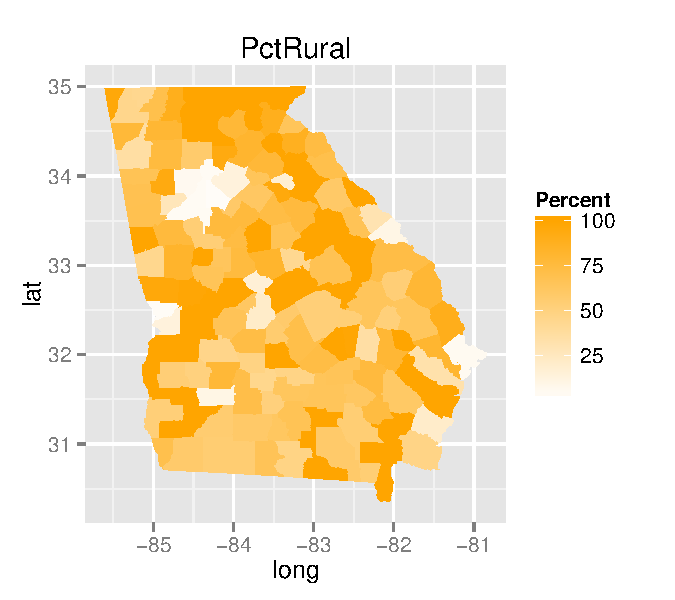
\includegraphics{figure/PctRural.pdf}
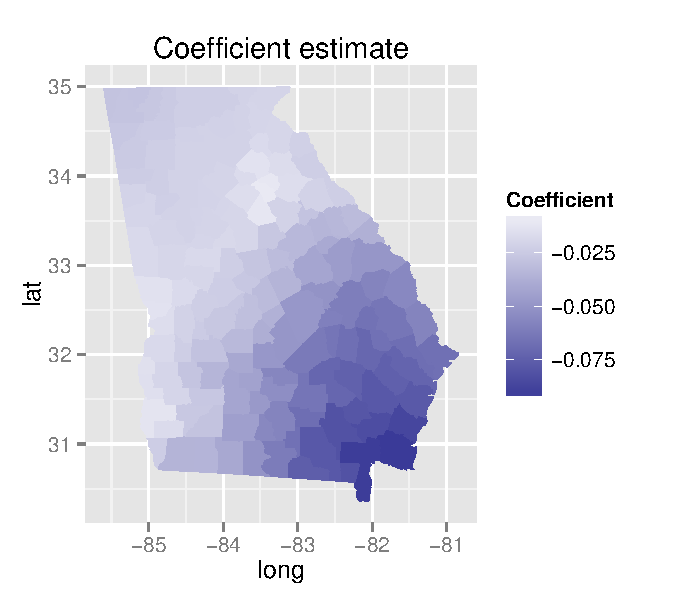
\includegraphics{figure/coef.pdf}
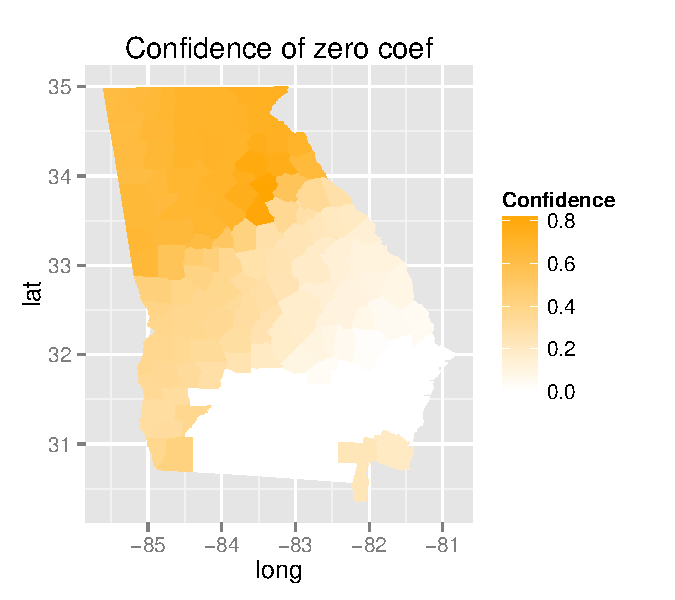
\includegraphics{figure/zero.pdf}
\end{adjustbox}
\caption{An example produced by the \code{plot.lagr()} function. Plots are based on a model for educational attainment by county in Georgia. The response is the PctBach, the percentage of residents in each county who have at least a bachelor's degree. Left: PctRural, the percentage of people in each county who live in a rural area. Middle: estimated coefficient of PctRural. Right: confidence that the coefficient of PctRural is exactly zero.}
\label{fig:georgia}
\end{widefigure}


\section{Summary}
This paper has outlined the varying coefficient regression model, and shown how local adaptive grouped regularization is used for local variable selection and estimation. The R package \pkg{lagr} was introduced and illustrated by estimating a model for educational attainment in Georgia. In particular, the \code{lagr.tune} function was used to estimate the model's bandwidth parameter, the \code{lagr} function was used to fit a model using the estimated bandwidth, and the \code{plot.lagr} function was used to produce choropleths of the results of analysis. 

\bibliography{references}

%\address{Wesley Brooks\\
%  Department of Statistics, University of Wisconsin-Madison\\
%  1300 University Ave. Madison, WI 53706\\
%  USA}
%\email{wrbrooks@uwalumni.com}

